\documentclass[12pt, letterpaper]{article}

% Paquetes base
\usepackage[utf8]{inputenc}
\usepackage[spanish]{babel}
\usepackage{graphicx}
\usepackage{geometry}
\usepackage[table]{xcolor}
\usepackage{booktabs}
\usepackage{float}
\usepackage{tabularx}
\usepackage{array}
\usepackage{tikz}
\usetikzlibrary{babel,positioning,arrows.meta,shapes.geometric,calc}
\geometry{letterpaper, margin=2.5cm}

% Cabeceras y pie de página
\usepackage{fancyhdr}
\pagestyle{fancy}
\fancyhf{}
\fancyhead[L]{CoProof - Primer Parcial}
\fancyhead[R]{David L., Daniel T., Emiliano F.}
\fancyfoot[C]{\thepage}
\setlength{\headheight}{15pt}

% Paquetes para código, cajas, bibliografía y glosarios
\usepackage{listings}
\usepackage{amssymb}
\usepackage{tcolorbox}
\usepackage{caption}
\usepackage[hidelinks]{hyperref}
\usepackage{csquotes}
\usepackage[backend=biber, style=apa]{biblatex}
\addbibresource{referencias.bib}
\usepackage[nowarn]{glossaries}
\makenoidxglossaries
\ExplSyntaxOn
\msg_redirect_name:nnn { glossaries } { presort } { none }
\ExplSyntaxOff
\newglossaryentry{latex}{
    name=LaTeX,
    description={Un sistema de preparación de documentos de alta calidad}
}

\newglossaryentry{biber}{
    name=Biber,
    description={Herramienta para procesar bibliografía con biblatex}
}

\newglossaryentry{tcolorbox}{
    name=tcolorbox,
    description={Paquete para crear cajas de contenido estilizadas en LaTeX}
}


\hypersetup{
    colorlinks=true,
    linkcolor=blue!60!black,
    citecolor=blue!60!black,
    urlcolor=blue!60!black
}

\addto\captionsspanish{%
    \renewcommand{\tablename}{Tabla}%
    \renewcommand{\figurename}{Figura}%
    \renewcommand{\listtablename}{Índice de tablas}%
    \renewcommand{\listfigurename}{Índice de figuras}%
}

\renewcommand{\lstlistingname}{Código}
\renewcommand{\lstlistlistingname}{Índice de código}

\definecolor{storyheaderbg}{HTML}{EAF4FF}
\definecolor{storycontentbg}{HTML}{FFFDF7}
\definecolor{storyline}{HTML}{B8C6D9}

\newcommand{\storycheck}[1]{\(\square\)~#1\par}

\newcommand{\story}[3]{%
\begin{table}[H]
    \centering
    \begingroup
    \arrayrulecolor{storyline}
    \setlength{\tabcolsep}{10pt}
    \renewcommand{\arraystretch}{1.55}
    \begin{tabularx}{\textwidth}{|>{\raggedright\arraybackslash\bfseries\columncolor{storyheaderbg}}p{3.4cm}|>{\raggedright\arraybackslash\columncolor{storycontentbg}}X|}
        \hline
        Título & #1 \\
        \hline
        Historia de usuario & #2 \\
        \hline
        Criterios de aceptación & #3 \\
        \hline
    \end{tabularx}
    \endgroup
\end{table}
}

% Configuración de numeración independiente (por sección si se desea)
\usepackage{chngcntr}
\counterwithin{figure}{section}
\counterwithin{table}{section}

% Configuración de Listings (Snippets de código)
\lstdefinestyle{codigo}{
    backgroundcolor=\color{gray!8},
    basicstyle=\ttfamily\small,
    keywordstyle=\color{blue!70!black}\bfseries,
    commentstyle=\color{green!40!black}\itshape,
    stringstyle=\color{orange!60!black},
    numberstyle=\tiny\color{gray!70!black},
    numbers=left,
    stepnumber=1,
    numbersep=8pt,
    frame=single,
    rulecolor=\color{gray!50},
    breaklines=true,
    showstringspaces=false,
    tabsize=4,
    captionpos=b
}
\lstset{style=codigo}

\begin{document}

% --- PORTADA ---
\begin{titlepage}
    \centering
    
\includegraphics[width=0.28\textwidth]{img/ceti_logo.png}\par\vspace{1cm}
    
    {\scshape\LARGE CETI Plantel Colomos \par}
    \vspace{1cm}
    {\scshape\Large Aseguramiento de la Calidad de Software \par}
    \vspace{1.5cm}
    {\huge\bfseries CoProof\\Documentos Primer Parcial \par}
    \vspace{1.5cm}

    {\Large Profesor:\par}
    Luis Fernando Gaspar Pérez\par
    \vspace{1cm}
    
    {\Large Autores:\par}
    David Alejandro López Torres - 22310432\\ Daniel Tejeda Saavedra 22310431\\ Emiliano Flores Márquez 22110044\par
    \vspace{2cm}
    
    Guadalajara, México \par
    \vfill
    {\large \today \par}
\end{titlepage}

% --- ÍNDICE ---
\newpage
\tableofcontents
\listoftables
\listoffigures
% \lstlistoflistings
\newpage

% --- CONTENIDO ---
\section{Historias de usuario del sistema CoProof}

Las historias de usuario presentadas a continuación articulan los requisitos funcionales de CoProof desde la perspectiva del usuario final. Cada historia sigue un formato estructurado que incluye el actor (``Como''), la capacidad deseada (``quiero'') y el beneficio esperado (``para''), junto con criterios de aceptación explícitos que representan el contrato de calidad que el sistema debe cumplir. Esta estructura permite al equipo de desarrollo priorizar e iterar sobre capacidades de forma coherente, asegurando que cada incremento incremente valor percibido y mantenga consistencia de experiencia de usuario.

\subsection{Historias de autenticación y acceso}

\story
{Registro de cuenta}
{\textbf{Como} persona nueva en la plataforma, \textbf{quiero} crear una cuenta con correo verificable, \textbf{para} acceder al sistema con identidad propia.}
{%
\storycheck{El usuario completa formulario con teclado físico, teclado en pantalla o comando de voz asistido, y confirma con clic, toque o tecla Enter.}
\storycheck{Si falta un campo obligatorio, la interfaz muestra error en línea bajo el campo y un banner superior con resumen de errores.}
\storycheck{Si el correo ya existe, el sistema abre un diálogo modal con la opción de ir a iniciar sesión.}
\storycheck{La verificación se confirma por correo electrónico y se refleja en un panel de estado integrado en la vista de registro.}
\storycheck{Al finalizar, aparece un toast de éxito y el sistema redirige a la pantalla de inicio de sesión.}}

\story
{Inicio de sesión}
{\textbf{Como} usuario registrado, \textbf{quiero} iniciar sesión con correo y contraseña, \textbf{para} usar funciones que requieren autenticación.}
{%
\storycheck{El usuario ingresa credenciales con teclado físico, teclado en pantalla o comando de voz y envía con botón, Enter o comando ``iniciar''.}
\storycheck{Si las credenciales son correctas, el sistema abre el panel principal y muestra un toast de bienvenida con el rol activo.}
\storycheck{Si las credenciales son incorrectas, aparece un mensaje en línea bajo contraseña y un contador de intentos en un panel informativo.}
\storycheck{Tras 3 intentos fallidos, el sistema muestra diálogo de bloqueo temporal y acceso directo a recuperación de cuenta.}
\storycheck{Si hay error de conexión, el sistema muestra un banner persistente con opción ``Reintentar''.}}

\subsection{Historias de gestión de proyectos}

\story
{Creación de proyecto privado}
{\textbf{Como} usuario autenticado, \textbf{quiero} crear un proyecto privado, \textbf{para} trabajar con acceso restringido a colaboradores seleccionados.}
{%
\storycheck{El usuario abre ``Nuevo proyecto'', selecciona ``Privado'' y completa campos con teclado, ratón o pantalla táctil.}
\storycheck{El sistema valida campos requeridos y muestra errores en línea antes de permitir confirmar.}
\storycheck{Al crear, el sistema asigna al creador como líder y muestra diálogo de confirmación con identificador del proyecto.}
\storycheck{La invitación de colaboradores se realiza desde un panel lateral con búsqueda por correo o nombre.}}

\subsection{Historias de sesión abierta}

\story
{Apertura de proyecto en sesión individual}
{\textbf{Como} usuario con acceso autorizado, \textbf{quiero} abrir un proyecto en sesión individual, \textbf{para} trabajar en modo personal sobre el grafo.}
{%
\storycheck{El usuario selecciona un proyecto con doble clic, toque o comando ``abrir en sesión individual''.}
\storycheck{El sistema valida permisos y carga la vista del proyecto con indicador de modo en la barra superior.}
\storycheck{Si el acceso es denegado, se muestra diálogo modal con motivo y opción para solicitar acceso.}}

\subsection{Historias de validación}

\story
{Solicitud de demostración de nodo a un agente}
{\textbf{Como} usuario, \textbf{quiero} solicitar a un agente una demostración completa de un nodo, \textbf{para} evaluar una solución automática.}
{%
\storycheck{El usuario inicia la solicitud desde botón ``Pedir demostración'' en el panel del nodo.}
\storycheck{El sistema muestra cola y progreso en la consola integrada con estados: en cola, ejecutando, validando, finalizada.}
\storycheck{Si el agente entrega una propuesta, el sistema la presenta en el visor y muestra resultado de validación formal.}}

\story
{Guardado de cambios en sesión individual}
{\textbf{Como} usuario en sesión individual, \textbf{quiero} guardar cambios del proyecto, \textbf{para} crear una solicitud de autorización para el líder.}
{%
\storycheck{El usuario activa ``Guardar cambios'' con clic, toque, \texttt{Ctrl+S} o comando de voz habilitado.}
\storycheck{El sistema compila un resumen de cambios y lo muestra en un diálogo de confirmación antes del envío.}
\storycheck{Al confirmar, el sistema registra la solicitud y muestra identificador en un toast y en panel de actividad.}}

\clearpage

\section{Arquitectura}

\subsection{Visión general}

La plataforma CoProof está diseñada bajo un enfoque de \textbf{Arquitectura Orientada a Servicios (SOA, \textit{Service-Oriented Architecture})} con una transición progresiva hacia \textbf{microservicios} especializados. La decisión técnica central consiste en desacoplar las operaciones administrativas de las operaciones de validación formal asíncrona, debido a que el dominio del problema ---la verificación formal de teoremas y la compilación de proyectos matemáticos en Lean4--- presenta cargas de trabajo costosas, de duración variable y con picos de latencia difíciles de predecir. En este contexto, un diseño monolítico síncrono degradaría rápidamente la experiencia de usuario cuando múltiples validaciones se ejecutan de forma concurrente.\\

El principio operativo principal es el \textbf{procesamiento asíncrono impulsado por eventos}. En términos prácticos, el \textbf{Backend Core} administra estado y reglas de negocio, mientras que el \textbf{Lean Worker} procesa tareas de compilación y validación formal fuera del ciclo de petición-respuesta inmediato. Esta separación se alinea con una aplicación de \textbf{segregación de responsabilidades de consulta y comando (CQRS, \textit{Command Query Responsibility Segregation}) a nivel arquitectónico}: las rutas transaccionales y de lectura del dominio permanecen disponibles incluso cuando existen validaciones largas en cola.\\

La plataforma adopta una comunicación basada en mensajes mediante el patrón \textbf{publicación/suscripción (Pub/Sub, \textit{Publish/Subscribe})} y colas de trabajo. En lugar de acoplar Backend Core y Lean Worker con llamadas directas \textbf{RPC (\textit{Remote Procedure Call})} o flujos \textbf{HTTP (\textit{HyperText Transfer Protocol})} síncronos, se utiliza Redis como \textit{broker} de mensajes y almacén de resultados. Esta estrategia proporciona tolerancia a fallos: si un trabajador cae, la tarea no se pierde, sino que permanece encolada hasta que un proceso de worker vuelve a estar en línea y la consume. Además, el uso de identificadores de trabajo permite observabilidad y trazabilidad extremo a extremo.\\

Otro componente estructural es el \textbf{Gateway de Integración Externa}. CoProof no opera como almacenamiento aislado del código fuente, sino como orquestador entre: (1) un almacenamiento relacional para metadatos y estado del grafo de demostración, y (2) un motor externo de control de versiones (GitHub) que conserva el historial inmutable de cambios colaborativos. En consecuencia, la plataforma separa responsabilidades entre persistencia del estado lógico interno y versionado distribuido del contenido formal, evitando inconsistencias entre colaboración matemática y gestión de repositorios.

\subsection{Acrónimos y convención de notación}

Para mantener consistencia en todo el documento, se utiliza la siguiente notación estable:
\begin{itemize}
    \item \textbf{API}: Interfaz de Programación de Aplicaciones (\textit{Application Programming Interface}).
    \item \textbf{SOA}: Arquitectura Orientada a Servicios.
    \item \textbf{CQRS}: Segregación de responsabilidades de consulta y comando.
    \item \textbf{SPA}: Aplicación de Página Única (\textit{Single-Page Application}).
    \item \textbf{SSE}: Eventos Enviados por el Servidor (\textit{Server-Sent Events}).
    \item \textbf{REST}: Transferencia de Estado Representacional (\textit{Representational State Transfer}).
    \item \textbf{JSON}: Notación de Objetos de JavaScript (\textit{JavaScript Object Notation}).
    \item \textbf{ORM}: Mapeo Objeto-Relacional (\textit{Object-Relational Mapping}).
    \item \textbf{CI/CD}: Integración Continua y Entrega/Despliegue Continuo.
    \item \textbf{JWT}: JSON Web Token, esquema de token firmado para autenticación.
    \item \textbf{OAuth}: protocolo abierto de autorización delegada.
    \item \textbf{UUID}: Identificador Universalmente Único (\textit{Universally Unique Identifier}).
    \item \textbf{NL2FL}: traducción de lenguaje natural a lenguaje formal (\textit{Natural Language to Formal Language}).
\end{itemize}

Cuando se mencione \textbf{Backend Core}, se refiere al servidor principal de orquestación del dominio. Cuando se mencione \textbf{Lean Worker}, se refiere al microservicio validador formal. Cuando se mencione \textbf{Frontend SPA}, se refiere al cliente web de la plataforma. Esta convención se conserva de forma uniforme en todas las secciones y en la interpretación de los diagramas. En el alcance actual de los diagramas no se modela un microservicio explícito de cómputo exhaustivo.

\subsection{Visión de flujo extremo a extremo}

El flujo arquitectónico completo puede resumirse así: una acción de usuario inicia en el Frontend SPA, llega al Backend Core por REST/JSON, se valida contra reglas del dominio y, si requiere verificación formal, se transforma en un mensaje de tarea enviado al broker Redis. El Lean Worker consume esa tarea, ejecuta Lean4 en un entorno controlado, transforma la salida en JSON estandarizado y la deposita en el backend de resultados. Posteriormente, el Backend Core expone el avance y estado final al Frontend SPA, incluyendo notificaciones en tiempo real por SSE. Este ciclo evita bloqueos en el servidor principal, mejora la escalabilidad horizontal y preserva una experiencia interactiva incluso ante compilaciones costosas.\\

En términos de evolución, la topología permite incorporar nuevos microservicios (por ejemplo, módulos de NL2FL o agentes de IA) sin romper la orquestación existente: basta con definir nuevas colas y agregar adaptadores cliente en el Backend Core. Por ello, la arquitectura no está cerrada a un único tipo de validación matemática, sino preparada para un ecosistema de servicios especializados que comparten contratos de mensajería consistentes.

\subsection{Componentes y responsabilidades}

\subsubsection{Backend Flask}

Actúa como punto de entrada HTTP y coordinador entre base de datos, GitHub y LeanServer.

\begin{itemize}
    \item expone endpoints de auth, proyectos, nodos y webhooks,
    \item aplica reglas de negocio en servicios (\texttt{ProjectService}, \texttt{AuthService}, \texttt{CompilerClient}),
    \item persiste estado de dominio en PostgreSQL (\texttt{NewProject}, \texttt{NewNode}, \texttt{User}),
    \item usa Redis/Celery para ejecución asíncrona.
\end{itemize}

\subsubsection{LeanServer}

Se encarga de la validación formal de código Lean en aislamiento.

\begin{itemize}
    \item consume tareas \texttt{tasks.verify\_snippet} y \texttt{tasks.verify\_project\_files},
    \item ejecuta Lean sobre archivos temporales,
    \item parsea mensajes de compilación,
    \item retorna una respuesta normalizada (\texttt{valid}, \texttt{errors}, tiempos y conteos).
\end{itemize}

\subsubsection{Integración con GitHub}

Se utiliza para autenticación OAuth y como repositorio remoto del contenido Lean.

\begin{itemize}
    \item OAuth para obtener identidad/token del usuario,
    \item API REST para crear repositorios, actualizar archivos y gestionar PRs,
    \item webhook \texttt{push} para disparar reindexado asíncrono.
\end{itemize}

\subsection{Patrones de diseño aplicados}

\subsubsection{Arquitectura por capas}

Organización en capas con dependencias dirigidas, donde cada capa expone contratos y concentra una responsabilidad: API (entrada/salida HTTP), servicios (orquestación), dominio/datos (estado persistente) e infraestructura (tecnología externa). Regla operativa: API → Servicios → Dominio/Infraestructura.

\subsubsection{Application Factory}

\texttt{create\_app} centraliza creación de la aplicación y registro de extensiones/blueprints, concentrando la configuración por entorno.

\subsubsection{Productor–consumidor con colas}

El backend publica tareas y workers especializados las consumen. Productores (\texttt{CompilerClient}), Consumidor Lean (\texttt{lean\_queue}), Broker (\textbf{Redis}).

\subsubsection{Adapter/Gateway de integraciones}

\texttt{CompilerClient} abstrae RPC por Celery, \texttt{AuthService} encapsula llamadas a GitHub.

\subsubsection{Transaction Script sobre Git}

\texttt{read\_only\_worktree(...)} para validación sin persistencia, \texttt{git\_transaction(...)} para edición y commit/push.

\subsubsection{Control de concurrencia}

\texttt{acquire\_project\_lock} y \texttt{acquire\_branch\_lock} evitan condiciones de carrera en operaciones Git concurrentes.

\subsubsection{Propagación de estado en árbol de nodos}

El estado de \texttt{NewNode} (\texttt{sorry}, \texttt{validated}) se propaga por reglas: una solución válida marca el nodo como \texttt{validated}, un split devuelve nodos a \texttt{sorry} hasta completar subpruebas.

\subsubsection{Sincronización orientada a eventos}

El webhook de GitHub (\texttt{push}) dispara reindexado asíncrono (\texttt{async\_reindex\_project}) con validación HMAC.

\subsection{Flujos operativos principales}

\subsubsection{Autenticación}

\begin{enumerate}
    \item Frontend solicita URL OAuth (\texttt{GET /api/v1/auth/github/url}).
    \item Usuario autoriza y frontend recibe \texttt{code}.
    \item Frontend envía \texttt{code} a backend (\texttt{POST /api/v1/auth/github/callback}).
    \item \texttt{AuthService} intercambia token y emite JWT interno.
    \item Renovación con refresh token (\texttt{POST /api/v1/auth/refresh}).
\end{enumerate}

\subsubsection{Creación de proyecto}

\begin{enumerate}
    \item Frontend envía \texttt{POST /api/v1/projects}.
    \item \texttt{ProjectService} valida datos y token GitHub.
    \item Se valida contexto Lean del objetivo con \texttt{CompilerClient.verify\_snippet}.
    \item Se crea repositorio remoto con archivos iniciales.
    \item Se persisten \texttt{NewProject} y nodo raíz \texttt{NewNode}.
\end{enumerate}

\subsubsection{Validación de nodo (solve)}

\begin{enumerate}
    \item Frontend envía \nolinkurl{POST /api/v1/projects/{project_id}/nodes/{node_id}/solve}.
    \item \texttt{nodes.solve\_node} reconstruye contexto por árbol de imports.
    \item Se verifica con LeanServer.
    \item Si es válido, se crea rama y pull request.
\end{enumerate}

\subsection{Modelo de dominio}

\subsubsection{Entidades principales}

\begin{itemize}
    \item \texttt{NewProject}: datos del proyecto, configuración de objetivo, repositorio remoto y colaboradores.
    \item \texttt{NewNode}: unidad de trabajo en el DAG lógico, con jerarquía padre-hijo y estado.
    \item \texttt{User}: identidad local y vínculo OAuth/token con GitHub.
\end{itemize}

\subsubsection{Relaciones clave}

\begin{itemize}
    \item \texttt{NewProject} 1..* \texttt{NewNode}.
    \item \texttt{NewNode} tiene autorrelación (\texttt{parent} / \texttt{children}).
    \item \texttt{User} se vincula a proyectos por autoría y colaboración.
\end{itemize}

\clearpage

\section{Diagrama de clases}

\subsection{Diagrama de clases del servidor (Backend Core)}

El diagrama de clases \textbf{class-01} representa al Backend Core como cerebro administrativo de la plataforma. Su propósito principal no es ejecutar lógica matemática de Lean4, sino coordinar recursos de dominio, validar permisos, mantener consistencia transaccional y actuar como punto de integración entre clientes, base de datos y sistema de colas. Esta distinción funcional es crítica: al evitar ejecutar validaciones formales prolongadas dentro del proceso principal, el servidor conserva capacidad de respuesta para autenticación, navegación de grafos y operaciones de colaboración.

\subsection{Capa de runtime y configuración}

El diseño del runtime utiliza un patrón \textbf{Factory} mediante \texttt{AppFactory}, apoyado por un \texttt{ConfigResolver} para inyectar configuración por entorno. El diagrama distingue explícitamente una configuración de pruebas (\texttt{TestingConfig}, con SQLite en memoria) y una configuración productiva (\texttt{ProductionConfig}, con PostgreSQL), lo que respalda un pipeline de CI/CD robusto y reproducible. Esta separación de entornos reduce riesgos de regresión al permitir pruebas rápidas y aisladas sin depender de infraestructura externa persistente.\\

Adicionalmente, un \texttt{ExtensionRegistry} centraliza extensiones transversales del servicio: \textbf{SQLAlchemy} como ORM, \textbf{Alembic} para migraciones de esquema y extensiones de autenticación basadas en JWT. Este registro evita inicializaciones dispersas y mejora la mantenibilidad porque concentra el punto de acoplamiento técnico en una sola capa de arranque.

\subsection{Capa de API}

La capa de API sigue un enrutamiento estandarizado y expone recursos orientados al dominio de pruebas formales. En particular, \texttt{NodesController} concentra endpoints de alto valor funcional, como \texttt{solve\_node}, \texttt{split\_node} y \texttt{verify\_node\_import\_tree}. La presencia de estas operaciones en el diagrama evidencia que el servidor no gestiona únicamente entidades CRUD tradicionales, sino transformaciones sobre estructuras jerárquicas de metas, submetas y dependencias de importación.\\

Desde la perspectiva arquitectónica, estas rutas constituyen una interfaz semántica sobre grafos de demostración. Es decir, cada endpoint no solo muta registros, sino que preserva invariantes del árbol de prueba colaborativo: coherencia entre nodos padre e hijo, control de prerrequisitos y estados de validación compatibles con la estrategia de compilación formal.

\subsection{Capa de servicios}

La lógica de negocio vive en servicios de dominio. \texttt{LeanService} prepara cargas útiles de verificación mediante \texttt{build\_verify\_payload} y normaliza importaciones por \texttt{normalize\_lean\_imports} antes de delegar la validación formal asíncrona. Esta prevalidación protege al sistema de inconsistencias sintácticas y evita enviar al worker datos mal estructurados.\\

Para asincronía, el diagrama muestra el patrón \textbf{Client/Adapter} con \texttt{CompilerClient}. Este cliente encapsula la complejidad de encolado en Redis vía \texttt{dispatch\_task} y devuelve un identificador de trabajo que sirve para rastreo posterior. El beneficio es doble: desacopla el backend de la implementación concreta del worker y permite evolucionar la infraestructura de ejecución sin rediseñar los controladores REST.

\subsection{Modelos y esquemas}

En la capa de persistencia, destaca \texttt{GraphNodeModel} con identificadores UUID, un campo de clasificación de nodo (\texttt{node\_type}: \texttt{global}, \texttt{goal}, \texttt{theorem}, \texttt{lemma}) y relaciones jerárquicas complejas (\texttt{parent}, \texttt{children}, \texttt{prerequisites}). Esta modelación facilita construir árboles de demostración colaborativos donde cada nodo representa una pieza verificable y trazable del proceso formal.\\

Los \textit{schemas} (implementados con Marshmallow) actúan como capa anticorrupción para serialización y deserialización hacia el Frontend SPA. En otras palabras, aíslan el modelo interno del contrato externo, permitiendo cambios internos en persistencia sin romper la interfaz de consumo.\\

En conjunto, \textbf{class-01} muestra una arquitectura backend madura: configuración desacoplada por entorno, controladores orientados al dominio, servicios de normalización y adaptación asíncrona, y una capa de datos capaz de representar colaboraciones matemáticas complejas de forma consistente.

\clearpage
\begin{figure}[p]
    \centering
    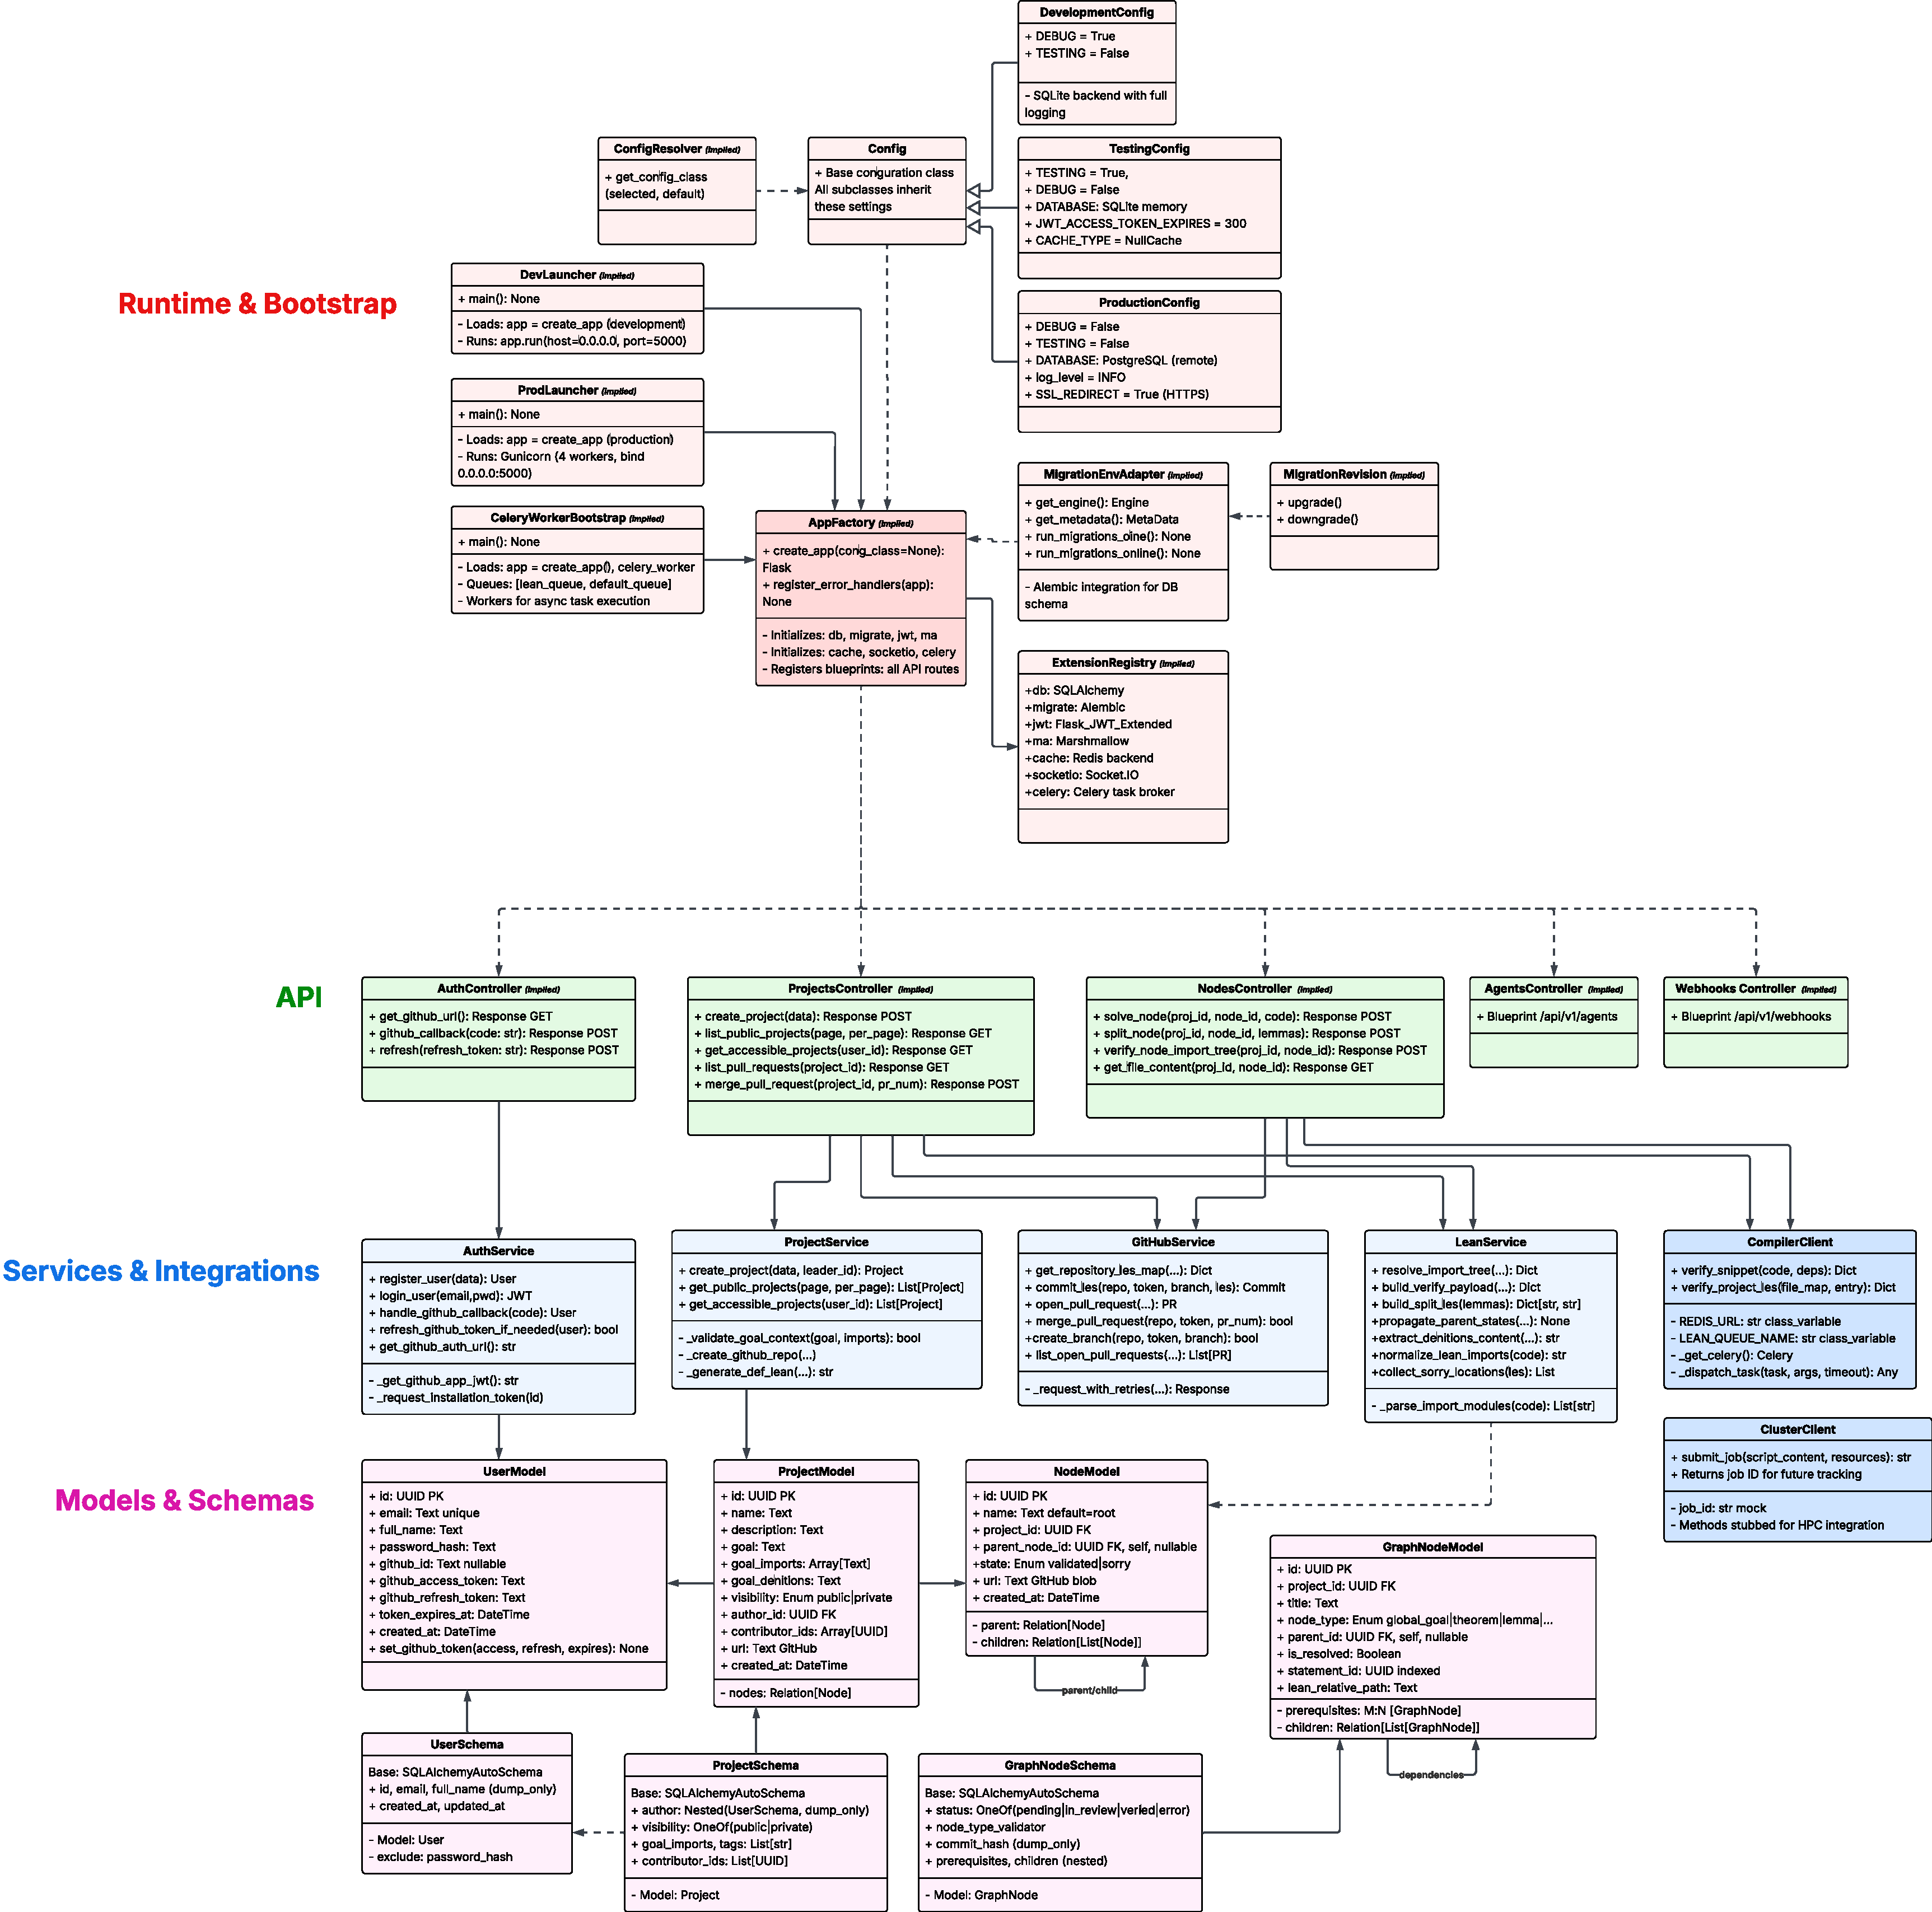
\includegraphics[width=\textwidth,keepaspectratio]{img/class-01.pdf}
    \caption{Diagrama de clases del servidor}
    \label{fig:diagrama-clases-servidor}
\end{figure}

\clearpage

\subsection{Diagrama de clases del Lean Worker (microservicio)}

El diagrama \textbf{class-02} describe el microservicio Lean Worker como un proceso \textbf{sin estado} orientado a validación formal. A diferencia del Backend Core, este componente no expone puertos HTTP ni administra sesiones de usuario; su responsabilidad es consumir tareas de verificación, ejecutar Lean4 de forma controlada y devolver resultados estructurados. Esta separación reduce superficie de fallo y simplifica el escalado horizontal: agregar capacidad equivale a instanciar más workers escuchando la misma cola.\\

Es importante precisar el alcance: en la versión actual de los diagramas, el Lean Worker representa el \textbf{validador formal} y no un microservicio independiente de cómputo exhaustivo. Si en una iteración futura se añade ese tipo de servicio, deberá modelarse como componente adicional con su propia cola, contratos y adaptador en el Backend Core.

\subsection{Inicialización y enrutamiento}

La inicialización del servicio se realiza mediante \texttt{LeanWorkerLauncher}. El enrutamiento no se basa en endpoints REST, sino en colas de Celery (por ejemplo, \texttt{lean\_queue}) definidas en \texttt{LeanWorkerConfig}. En este modelo, el \texttt{LeanTasksController} registra manejadores de comandos explícitos, como \texttt{verify\_snippet} y \texttt{verify\_project\_files}. Esta interfaz orientada a tareas evita ambigüedad de entrada y favorece contratos de payload fuertemente tipados por operación.\\

El uso de comandos discretos también permite establecer políticas diferenciadas de tiempo de ejecución, validación de parámetros y trazabilidad por tipo de tarea. Así, el worker conserva un comportamiento predecible incluso cuando conviven validaciones de distinta complejidad en la misma infraestructura.

\subsection{Servicios}

\texttt{LeanVerificationService} funciona como envoltorio directo del runtime formal. Sus responsabilidades incluyen localizar el ejecutable adecuado (\texttt{find\_lean\_executable}), lanzar procesos del sistema operativo y extraer resultados semánticos mediante \texttt{parse\_theorem\_info} y \texttt{parse\_lean\_messages}. Este último punto es especialmente relevante: la salida nativa de Lean no siempre es apta para consumo directo por API, por lo que el parseo estructurado transforma mensajes técnicos en información utilizable por el resto de la plataforma.\\

La estandarización de salida evita acoplar el Frontend SPA o el Backend Core a detalles internos del compilador. En consecuencia, cambios de formato en la herramienta formal se aíslan dentro del worker, preservando estabilidad de contratos externos.

\subsection{Gestión de entorno temporal}

Para validación de proyectos completos, \texttt{ProjectVerificationService} administra espacios de trabajo temporales (por ejemplo, \texttt{workspace\_tmp\_by\_file\_map}) y configura variables como \texttt{LEAN\_PATH}. También impone \textit{timeouts} estrictos (referencia operativa de 90 segundos) para evitar que pruebas infinitas, recursiones patológicas o entradas mal diseñadas bloqueen el worker indefinidamente.\\

Esta política de aislamiento temporal y límites de ejecución cumple tres objetivos: proteger recursos del host, evitar degradación acumulativa del clúster y ofrecer tiempos de respuesta máximos acotados para la capa de orquestación. En un sistema orientado a eventos, estos límites son indispensables para mantener cola saludable y prevenir efecto cascada de retrasos.

\subsection{Normalización}

El \texttt{CompilerAdapterService} convierte la salida de Lean a un \textbf{JSON} uniforme y consumible por el Backend Core. Esta etapa cierra la frontera técnica entre ejecución formal y orquestación de dominio: el worker se especializa en ejecutar y traducir, mientras el backend se especializa en decidir, persistir y publicar estados.\\

En síntesis, \textbf{class-02} muestra un validador formal robusto y escalable, con entrada por colas, ejecución aislada, control de tiempos, parseo semántico y salida estandarizada. El valor arquitectónico de este diagrama radica en su claridad de responsabilidades: la verificación formal queda encapsulada en un microservicio desacoplado del tráfico interactivo de la plataforma.

\clearpage
\begin{figure}[p]
    \centering
    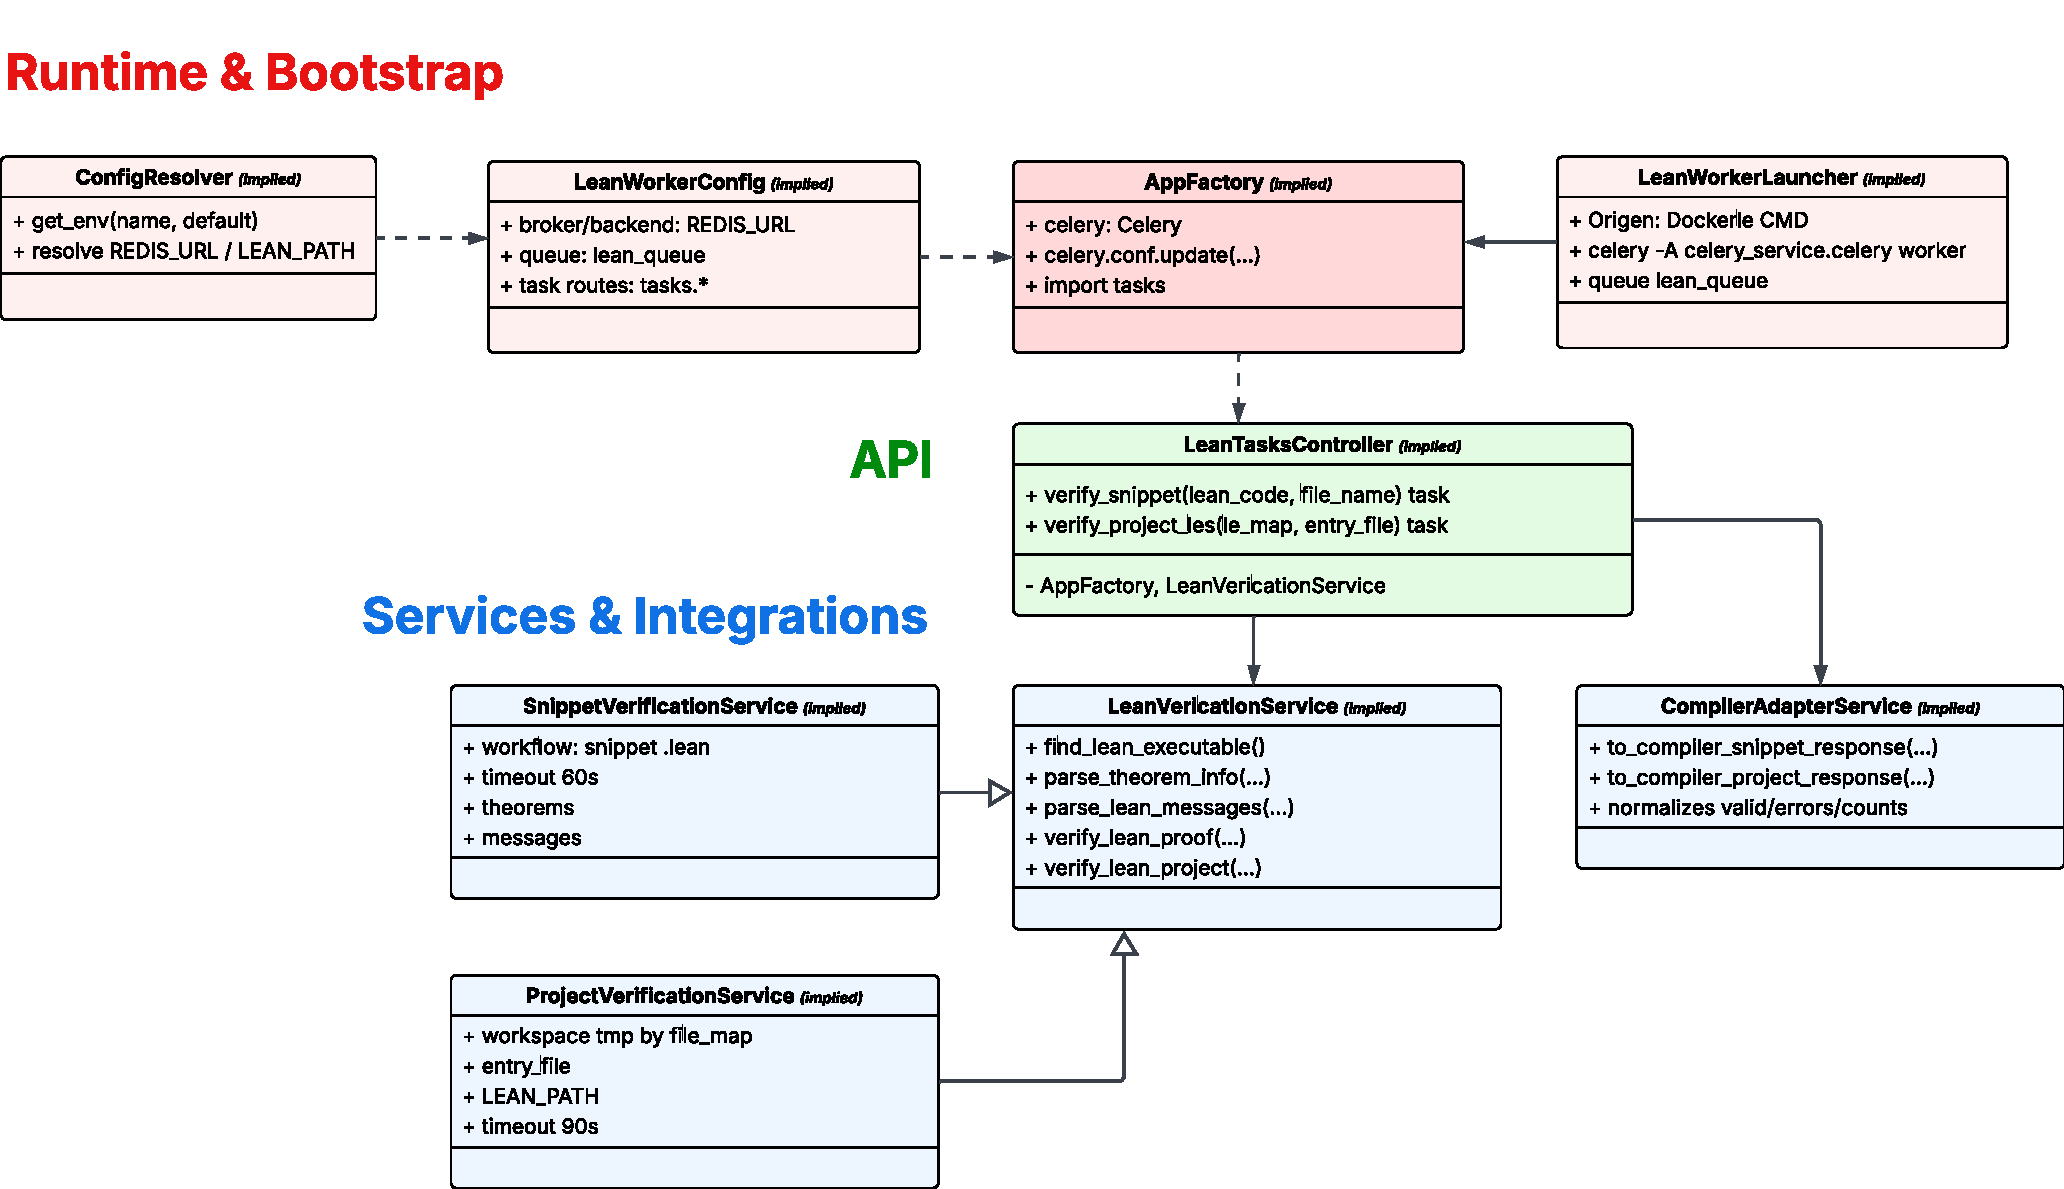
\includegraphics[width=\textwidth,keepaspectratio]{img/class-02.pdf}
    \caption{Diagrama de clases del Lean Server (microservicio)}
    \label{fig:diagrama-clases-lean}
\end{figure}

\clearpage

\subsection{Diagrama de clases del Frontend SPA}

El diagrama \textbf{class-03} presenta una \textbf{SPA (Single-Page Application)} estructurada de forma reactiva y fuertemente tipada, donde la navegación, el estado asíncrono y la interacción con validaciones formales se integran en una sola experiencia de usuario. A nivel arquitectónico, este cliente no es un simple consumidor de endpoints, sino un coordinador de flujos de trabajo complejos sobre grafos de demostración colaborativa.

\subsection{Arquitectura de interfaz y composición de rutas}

La composición visual se organiza con un enrutador jerárquico (\texttt{RoutesRegistry} con \texttt{<router-outlet/>}) contenido dentro de un \texttt{ShellComponent}. El shell define el marco de navegación persistente y desacopla estructura de pantalla respecto a la lógica de cada página de dominio. Este patrón permite escalar vistas sin duplicar infraestructura de menú, control de sesión y layout general.\\

El valor de esta decisión es doble: mejora mantenibilidad del código frontend y ofrece una experiencia consistente para el usuario, aun cuando cambie de contexto entre módulos de proyecto, validación o administración.

\subsection{Componentes de dominio y operaciones principales}

Dentro del conjunto de páginas, \texttt{WorkspacePageComponent} actúa como núcleo funcional. Según el diagrama, ejecuta tareas como \texttt{loadGraph}, \texttt{parseGoalImports}, \texttt{verifyNode} y \texttt{solveNode}. Estas acciones evidencian que el frontend participa activamente en la preparación de contexto para validación formal, no únicamente en la presentación de resultados.\\

Por ejemplo, \texttt{loadGraph} organiza la visualización del estado lógico del proyecto; \texttt{parseGoalImports} prepara dependencias requeridas para compilar metas; y \texttt{verifyNode}/\texttt{solveNode} disparan operaciones de verificación y resolución con retorno asíncrono. La combinación de estas capacidades permite al usuario iterar sobre pruebas matemáticas con retroalimentación gradual y trazabilidad de cambios.

\subsection{Estado asíncrono y observabilidad en tiempo real}

Dado que la validación formal puede tardar desde segundos hasta intervalos mayores, el frontend implementa un patrón \textbf{Observer} a través de \texttt{TaskStreamService}. Este servicio mantiene una conexión persistente de \textbf{SSE} usando \texttt{EventSource} para recibir eventos del ciclo de vida de tareas: encolado, ejecución, éxito, error o expiración.\\

Con ello, la interfaz evita bloqueos visuales, elimina necesidad de sondeo agresivo y mejora transparencia del proceso para el usuario final. Desde el punto de vista arquitectónico, SSE funciona como puente entre la frontera asíncrona de colas y la experiencia interactiva de la SPA.

\subsection{Capa de comunicaciones y seguridad}

\texttt{HttpGatewayService} centraliza llamadas de red y construye cabeceras de autorización con JWT (por ejemplo, \texttt{authHeaders}). Este gateway se comunica con la API REST principal y con rutas de consulta de estado de workers cuando corresponde. Al concentrar acceso HTTP en un servicio único, el frontend reduce duplicación, mejora trazabilidad de errores y facilita aplicar políticas homogéneas de autenticación, reintentos y manejo de respuestas.\\

En resumen, \textbf{class-03} describe un frontend con responsabilidades claramente delimitadas: shell y rutas para estructura, componentes de dominio para flujo matemático, stream asíncrono para visibilidad de tareas y gateway de red para seguridad y consistencia operacional. Esta arquitectura de cliente está alineada con la naturaleza distribuida del sistema y con el requisito de interacción continua durante procesos de validación costosos.

\clearpage
\begin{figure}[p]
    \centering
    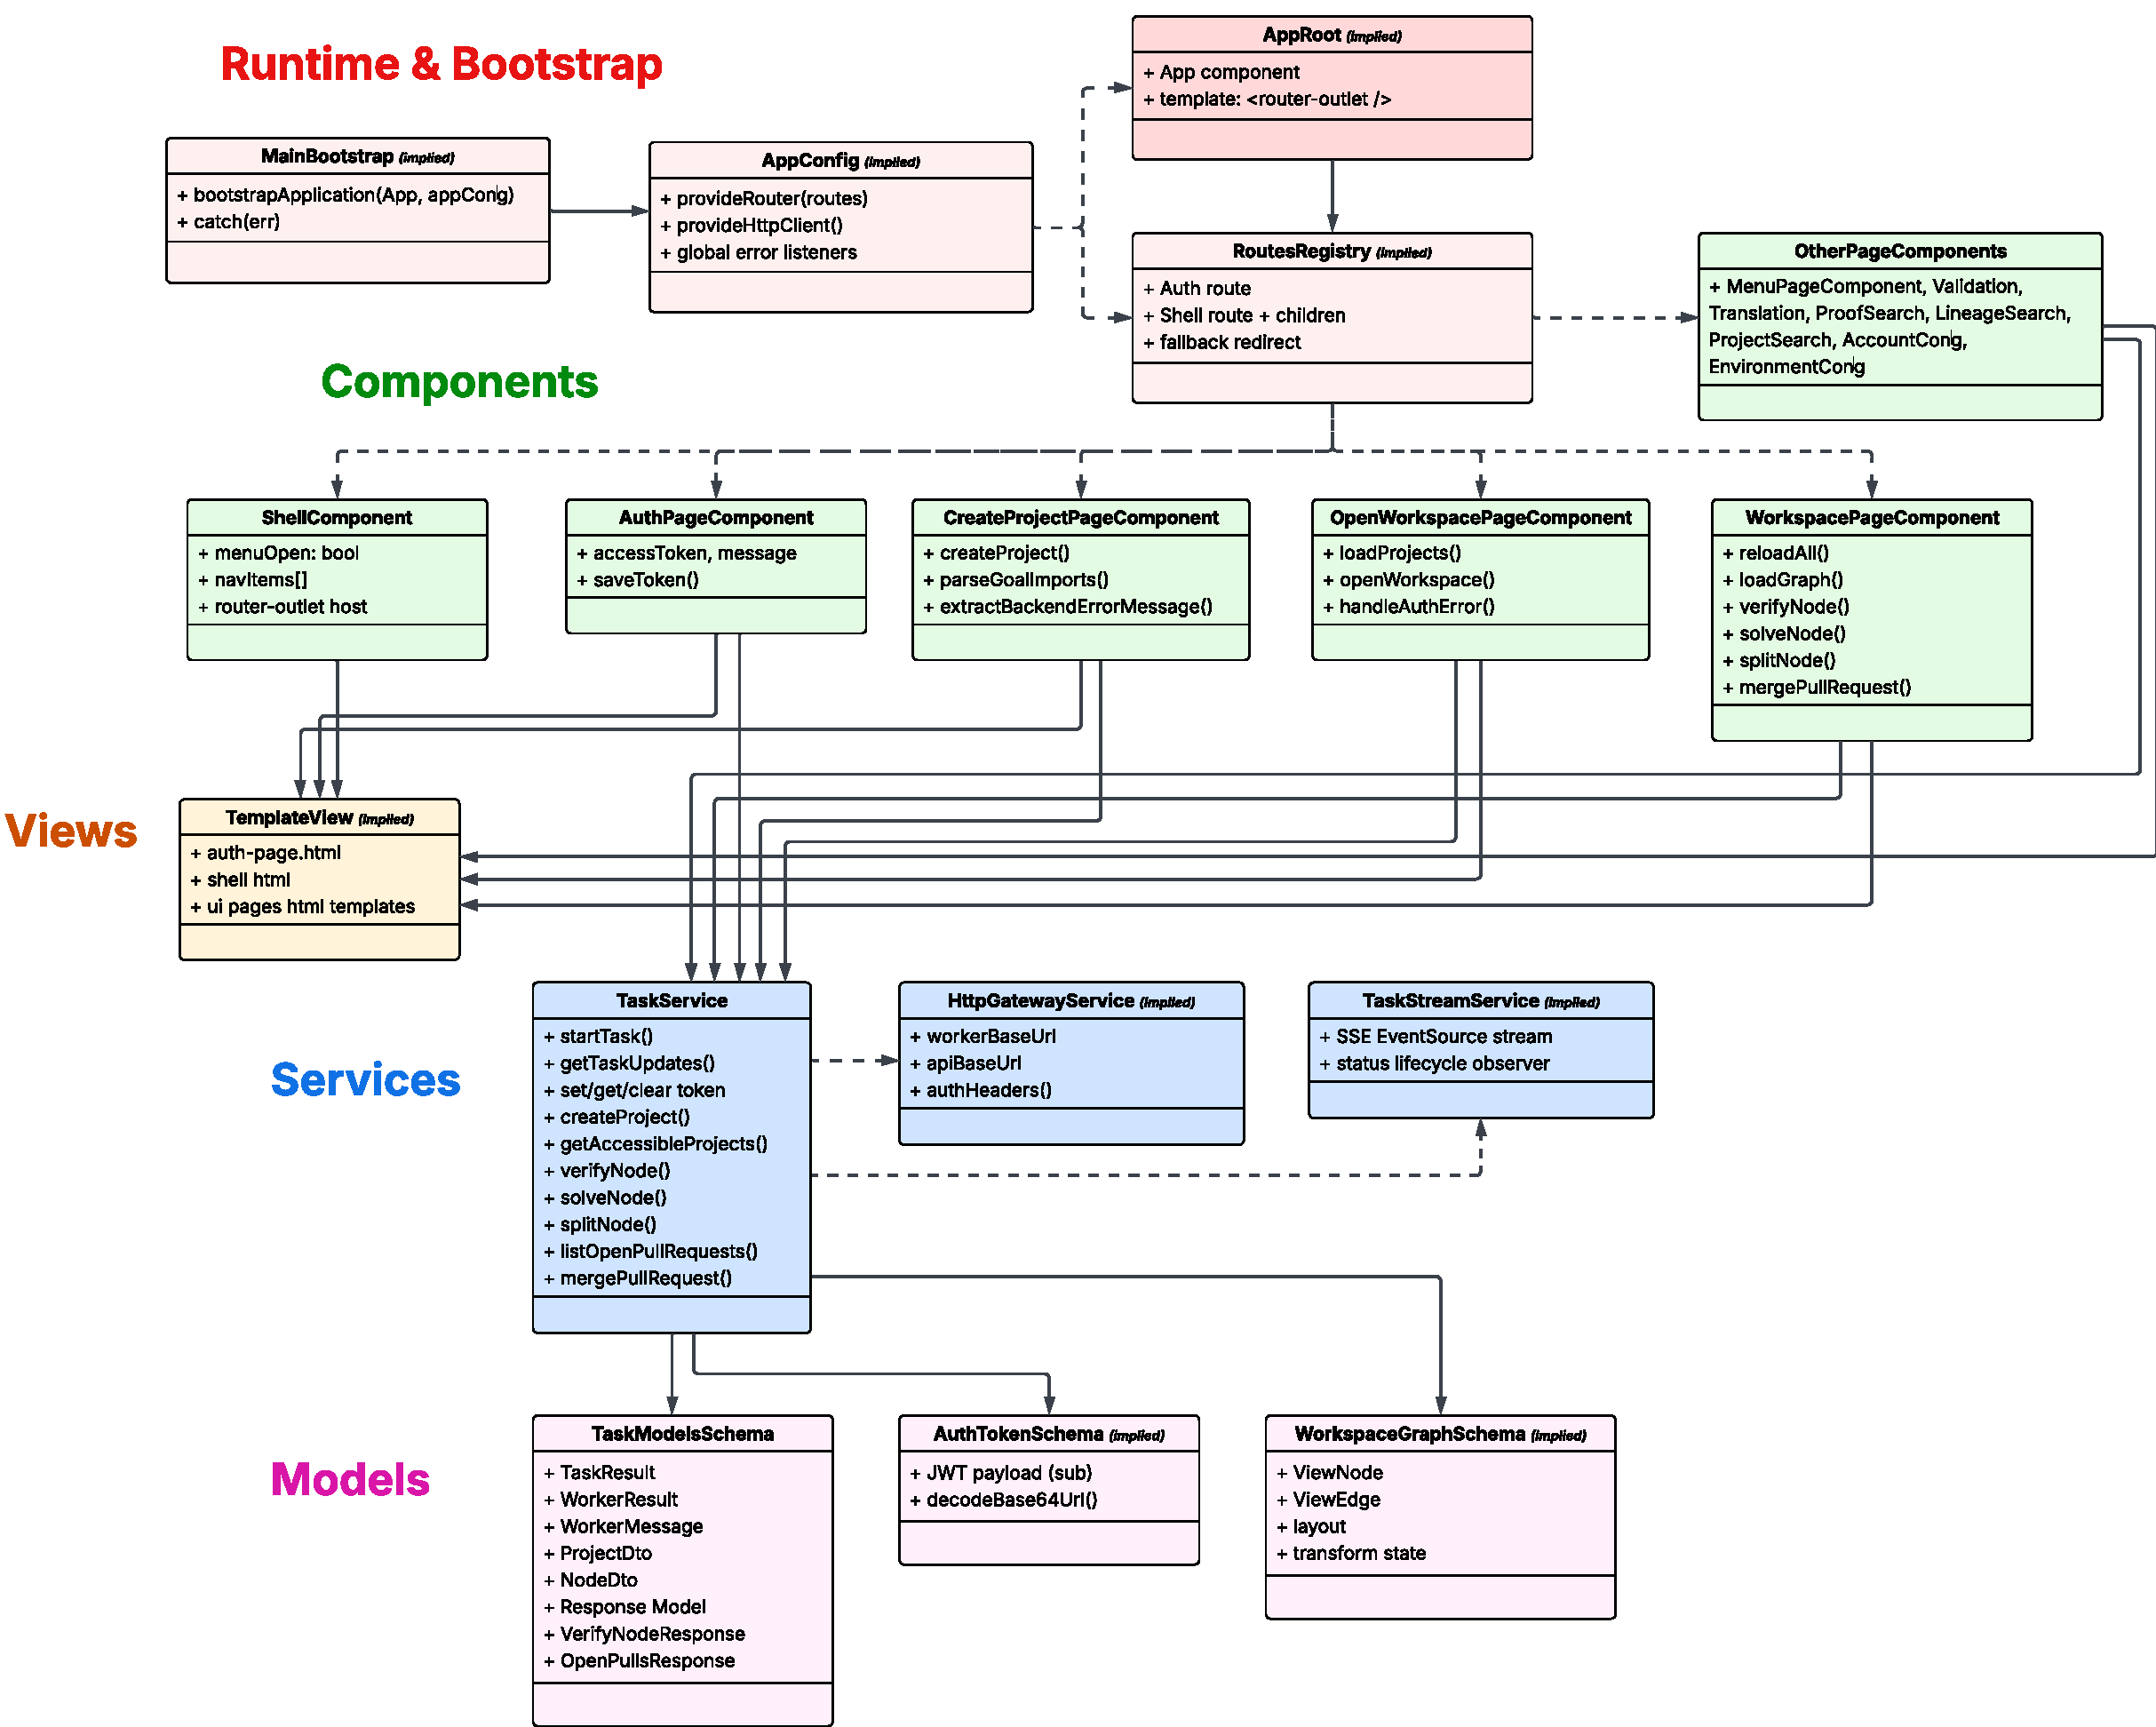
\includegraphics[width=\textwidth,keepaspectratio]{img/class-03.pdf}
    \caption{Diagrama de clases del Frontend}
    \label{fig:diagrama-clases-frontend}
\end{figure}

\clearpage

\section{Diagrama de calles}

El diagrama \textbf{street-01} muestra la topología de despliegue y las fronteras de comunicación de CoProof. A diferencia de los diagramas de clases, aquí el foco no es la estructura interna de objetos, sino el tránsito de información entre actores, contenedores y servicios. Esta perspectiva es esencial para validar propiedades no funcionales del sistema: latencia percibida, tolerancia a fallos, escalabilidad y aislamiento de cargas.

\subsection{Cliente a Backend Core}

La primera frontera conecta al usuario (Frontend SPA) con el Backend Core mediante \textbf{REST/HTTP} sobre \textbf{JSON}. En esta capa, el backend resuelve autenticación y autorización, incluyendo el flujo \textbf{OAuth} con GitHub, además de persistir estado estructural del dominio en PostgreSQL mediante ORM. Todo intercambio síncrono aquí está orientado a operaciones de control: abrir proyectos, consultar estructura de nodos, solicitar acciones de validación y recuperar estados de negocio.\\

Mantener esta frontera separada de la validación formal asíncrona permite tiempos de respuesta más estables en navegación y edición, aun si existen múltiples validaciones activas en segundo plano.

\subsection{Backend Core a Lean Worker}

Cuando una operación requiere validación formal, el Backend Core no ejecuta Lean directamente. En su lugar, delega el trabajo a través del \texttt{CompilerClient} (gateway interno de compilación), que emite un mensaje estructurado hacia Redis actuando como \textit{Message Broker} y \textit{Result Backend}. Este paso materializa el desacoplamiento arquitectónico: la petición del usuario se transforma en trabajo en cola con identidad propia y ciclo de vida independiente.\\

La ventaja clave es operativa: una caída temporal del worker no cancela la operación; simplemente retrasa su consumo. El sistema conserva así resiliencia frente a fallos del validador formal sin comprometer el canal principal de interacción.

\subsection{Resolución y retroalimentación}

El Celery Worker consume tareas de \texttt{lean\_queue} mediante un patrón \textit{pull}, ejecuta adaptadores de verificación de Lean y deposita resultados en Redis. Desde allí, el Backend Core consulta o recibe estados actualizados y los reenvía al Frontend SPA, incluyendo canales de eventos para actualización en tiempo real. Esta cadena de retorno completa el ciclo de una tarea asíncrona sin bloquear al usuario durante compilación.\\

El diagrama enfatiza que la experiencia de usuario no depende de una conexión de larga duración con el proceso de compilación; depende de un contrato de estado observable y consistente entre colas, backend y stream de eventos.

\subsection{Escalabilidad}

La topología también documenta la ruta de evolución del sistema. Integrar un traductor \textbf{NL2FL} o \textbf{agentes de IA} no exige rediseñar la arquitectura principal: basta con añadir contenedores de microservicios que escuchen nuevas colas (por ejemplo, \texttt{nl2fl\_queue}, \texttt{agent\_queue}) y crear un cliente adaptador adicional en el Backend Core, análogo a \texttt{CompilerClient}. Con ello, la orquestación permanece centralizada mientras la carga computacional se distribuye por dominio.\\

En términos de ingeniería de software, este diagrama de calles valida que CoProof está preparado para crecer por especialización de servicios, manteniendo límites claros entre coordinación, persistencia y ejecución formal. La consistencia de esta topología con los diagramas de clases confirma un diseño integral: el modelo lógico de software y el modelo físico de despliegue cuentan la misma historia arquitectónica.

\clearpage
\begin{figure}[p]
    \centering
    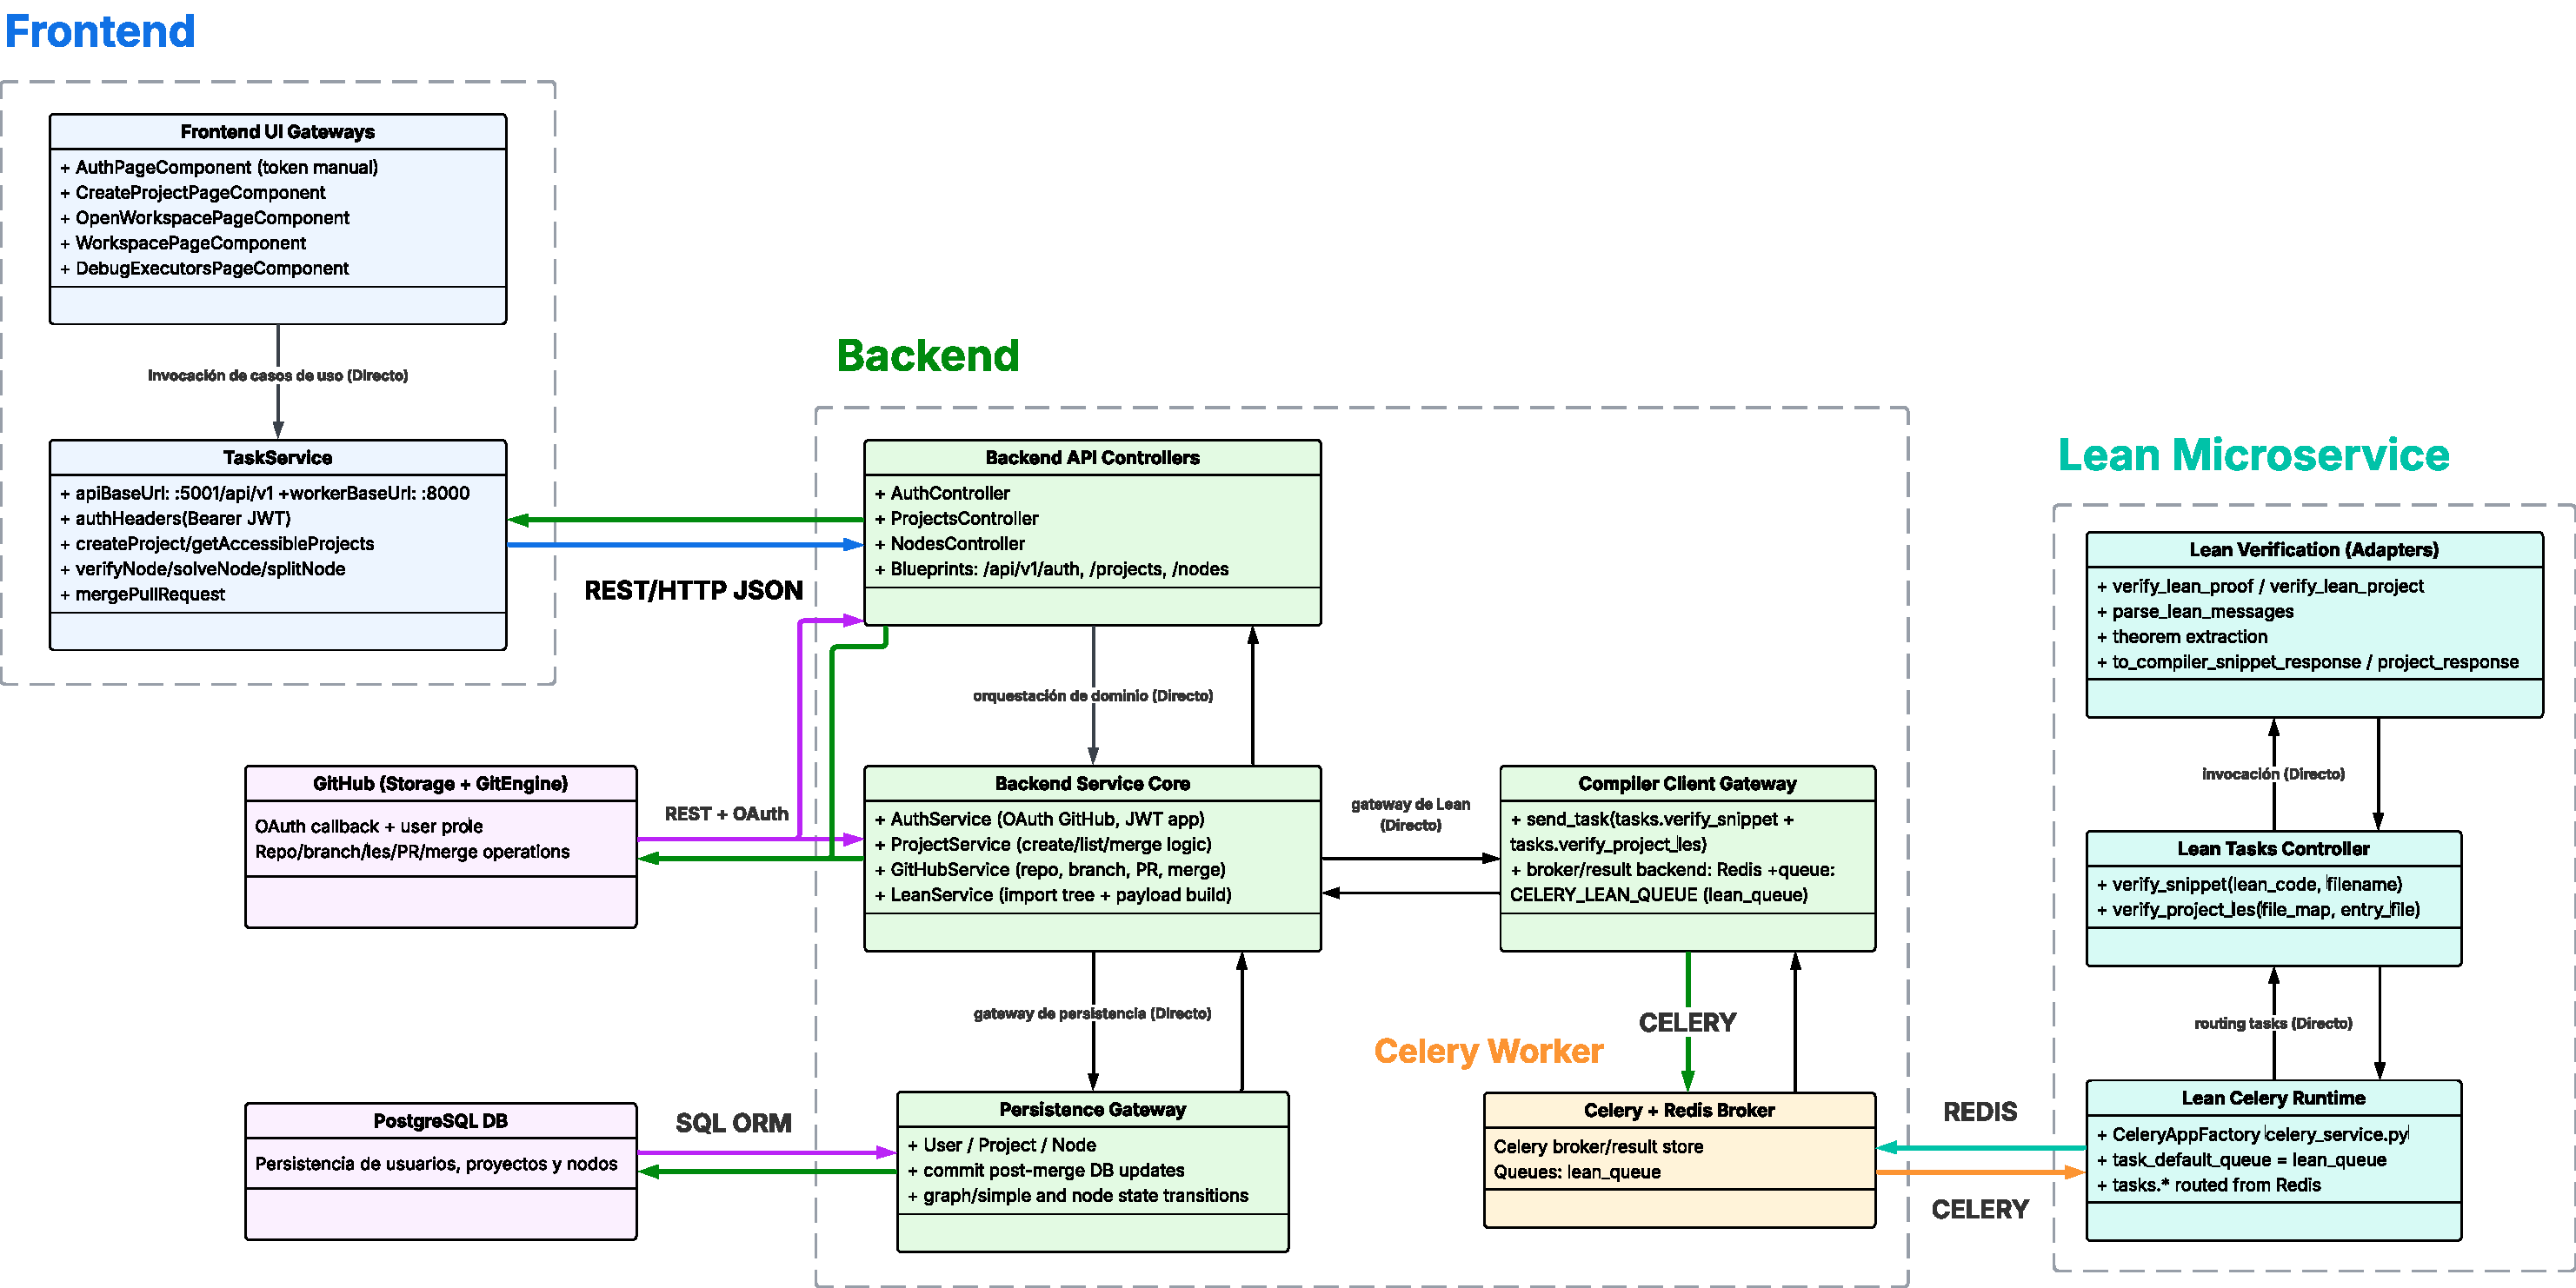
\includegraphics[width=\textwidth,keepaspectratio]{img/street-01.pdf}
    \caption{Diagrama de calles V1 (general)}
    \label{fig:diagrama-calles-v1}
\end{figure}

\clearpage
\begin{figure}[p]
    \centering
    \begingroup
    \shorthandoff{<>}
    \resizebox{\textwidth}{!}{\begin{tikzpicture}[
    x=1cm,
    y=1cm,
    >=Stealth,
    font=\fontsize{6}{6.8}\selectfont,
    service/.style={draw, rounded corners=2pt, align=center, minimum width=2.6cm, minimum height=1.0cm, fill=blue!8},
    external/.style={draw, rounded corners=2pt, align=center, minimum width=2.6cm, minimum height=1.0cm, fill=violet!10},
    db/.style={cylinder, shape border rotate=90, draw, align=center, minimum width=1.0cm, minimum height=2.4cm, aspect=0.3, fill=orange!15},
    flowbox/.style={draw, rounded corners=3pt, line width=0.5pt},
    msg/.style={midway, above, align=center, fill=white, inner sep=0.8pt, font=\fontsize{5}{5.8}\selectfont}
]

% --- Carriles (lifelines) ---
\node[service]  (frontend) at (0,0) {A - Frontend\\(SPA UI)\\TaskService / UI Gateways};
\node[external] (github)   at (3.55,0) {B - GitHub\\Servicio externo\\Storage + GitEngine};
\node[service]  (backend)  at (7.10,0) {C - Backend Gateway\\API Controllers\\Backend Service Core};
\node[db]       (pg)       at (10.65,0) {D - PostgreSQL\\DB relacional};
\node[db]       (redis)    at (14.20,0) {E - Redis\\Broker + Result Backend};
\node[service]  (worker)   at (17.75,0) {F - Lean Celery Worker\\Microservicio\\de validación};

\foreach \x in {0,3.55,7.10,10.65,14.20,17.75} {
    \draw[gray!65, densely dashed] (\x,-0.85) -- (\x,-26.9);
}

% --- Bloques de flujo ---
\draw[flowbox, blue!45]   (-1.8,-1.25) rectangle (19.55,-8.7);
\node[anchor=west, font=\bfseries\fontsize{6}{6.8}\selectfont, blue!55!black] at (-1.6,-1.55) {Flujo 1: Autenticación y sincronización de perfil (Síncrono externo)};

\draw[flowbox, teal!55!black] (-1.8,-9.2) rectangle (19.55,-14.9);
\node[anchor=west, font=\bfseries\fontsize{6}{6.8}\selectfont, teal!55!black] at (-1.6,-9.5) {Flujo 2: Modificación del grafo matemático (Transaccional interno)};

\draw[flowbox, red!55!black]  (-1.8,-15.4) rectangle (19.55,-26.6);
\node[anchor=west, font=\bfseries\fontsize{6}{6.8}\selectfont, red!55!black] at (-1.6,-15.7) {Flujo 3: Verificación de pruebas (Asíncrono desacoplado)};

% --- Flujo 1 ---
\draw[->, thick] (frontend.south |- 0,-2.2) -- (backend.south |- 0,-2.2)
    node[msg] {1.1 Login / validar token\\Vehículo: REST / HTTP JSON};

\draw[->, thick] (backend.south |- 0,-3.5) -- (github.south |- 0,-3.5)
    node[msg] {1.2 OAuth callback / perfil\\Vehículo: REST + OAuth};

\draw[->, thick, dashed] (github.south |- 0,-4.8) -- (backend.south |- 0,-4.8)
    node[msg] {1.3 Perfil + access tokens\\Vehículo: HTTP Response (JSON)};

\draw[->, thick] (backend.south |- 0,-6.1) -- (pg.south |- 0,-6.1)
    node[msg] {1.4 Upsert de usuario\\Vehículo: SQL ORM};

\draw[->, thick, dashed] (backend.south |- 0,-7.4) -- (frontend.south |- 0,-7.4)
    node[msg] {1.5 Sesión al cliente (JWT)\\Vehículo: HTTP Response + authHeaders};

% --- Flujo 2 ---
\draw[->, thick] (frontend.south |- 0,-10.2) -- (backend.south |- 0,-10.2)
    node[msg] {2.1 Caso de uso directo (ej. nuevo lema)\\Vehículo: REST / HTTP JSON + JWT};

\draw[->, thick] (backend.south |- 0,-11.5) -- (pg.south |- 0,-11.5)
    node[msg] {2.2 Actualizar nodo y transiciones\\Vehículo: SQL ORM};

\draw[<->, thick] (backend.south |- 0,-12.8) -- (github.south |- 0,-12.8)
    node[msg] {2.3 Commit y persistencia en rama\\Vehículo: REST API de GitHub};

\draw[->, thick, dashed] (backend.south |- 0,-14.1) -- (frontend.south |- 0,-14.1)
    node[msg] {2.4 Confirmación de éxito\\Vehículo: HTTP 200 OK};

% --- Flujo 3 ---
\draw[->, thick] (frontend.south |- 0,-16.4) -- (backend.south |- 0,-16.4)
    node[msg] {3.1 Solicitar verifyNode\\Vehículo: REST / HTTP JSON};

\draw[->, thick] (backend.south |- 0,-17.7) -- (redis.south |- 0,-17.7)
    node[msg] {3.2 Dispatch tasks.verify\_snippet / verify\_project\_files\\Vehículo: Protocolo Celery por lean\_queue};

\draw[->, thick, dashed] (backend.south |- 0,-19.0) -- (frontend.south |- 0,-19.0)
    node[msg] {3.3 Recepción inmediata + Job ID\\Vehículo: HTTP 202 Accepted};

\draw[->, thick] (redis.south |- 0,-20.3) -- (worker.south |- 0,-20.3)
    node[msg] {3.4 Consumo de tarea (routing)\\Vehículo: Suscripción asíncrona Celery Worker};

\draw[->, thick] (worker.south |- 0,-21.6) -- ++(1.0,0) -- ++(0,-1.0) -- ++(-1.0,0)
    node[pos=0.60, right, align=left, fill=white, inner sep=0.8pt, font=\fontsize{5}{5.8}\selectfont]
    {3.5 verify\_lean\_proof + parse\_lean\_messages\\Vehículo: Invocación directa (SO + adaptadores locales)};

\draw[->, thick] (worker.south |- 0,-23.1) -- (redis.south |- 0,-23.1)
    node[msg] {3.6 Guardar resultado formateado\\Vehículo: Celery Result Backend (Redis)};

\draw[->, thick] (backend.south |- 0,-24.4) -- (redis.south |- 0,-24.4)
    node[msg] {3.7 Leer resultado final\\Vehículo: Consulta directa a Redis};

\draw[->, thick, dotted] (backend.south |- 0,-25.7) -- (frontend.south |- 0,-25.7)
    node[msg] {3.8 Notificar tarea completada\\Vehículo: SSE / WebSockets o Webhook JSON};

\end{tikzpicture}
}
    \endgroup
    \caption{Diagrama de calles V2 (de flujos)}
    \label{fig:diagrama-calles-v2}
\end{figure}


% --- GLOSARIO Y BIBLIOGRAFÍA ---
% \clearpage
% \glsaddallunused
% \printnoidxglossary[title=Glosario,toctitle=Glosario]
% \clearpage
% \printbibliography[heading=bibintoc,title={Referencias}]

\end{document}
